\section{Technical Documentation}

The technical description of the ILD detector concept comprises specification and design documents as well as 3d engineering models, interface descriptions and drawings. All these documents that form the backbone of the ILD technical documentation are stored in the ILC Engineering Data Management System ILC-EDMS~\cite{ild:bib:edms}. As this powerful system is made for experts and requires appropriate attention, an easy accessible frontend ("EDMSdirect") has been made available. The ILD technical documentation is organised in a Work Breakdown Structure (WBS) that is mapped on a tree browser that can be accessed on the web~\cite{ild:bib:edmsdirect}. Figure~\ref{ild:fig:integration:edmsdirect} shows the tree browser for the ILD technical documentation. All WBS top nodes can be expanded by clicking on them. In the figure, this has been done for the node "Design Integration".


\begin{figure}[t!]
\centering
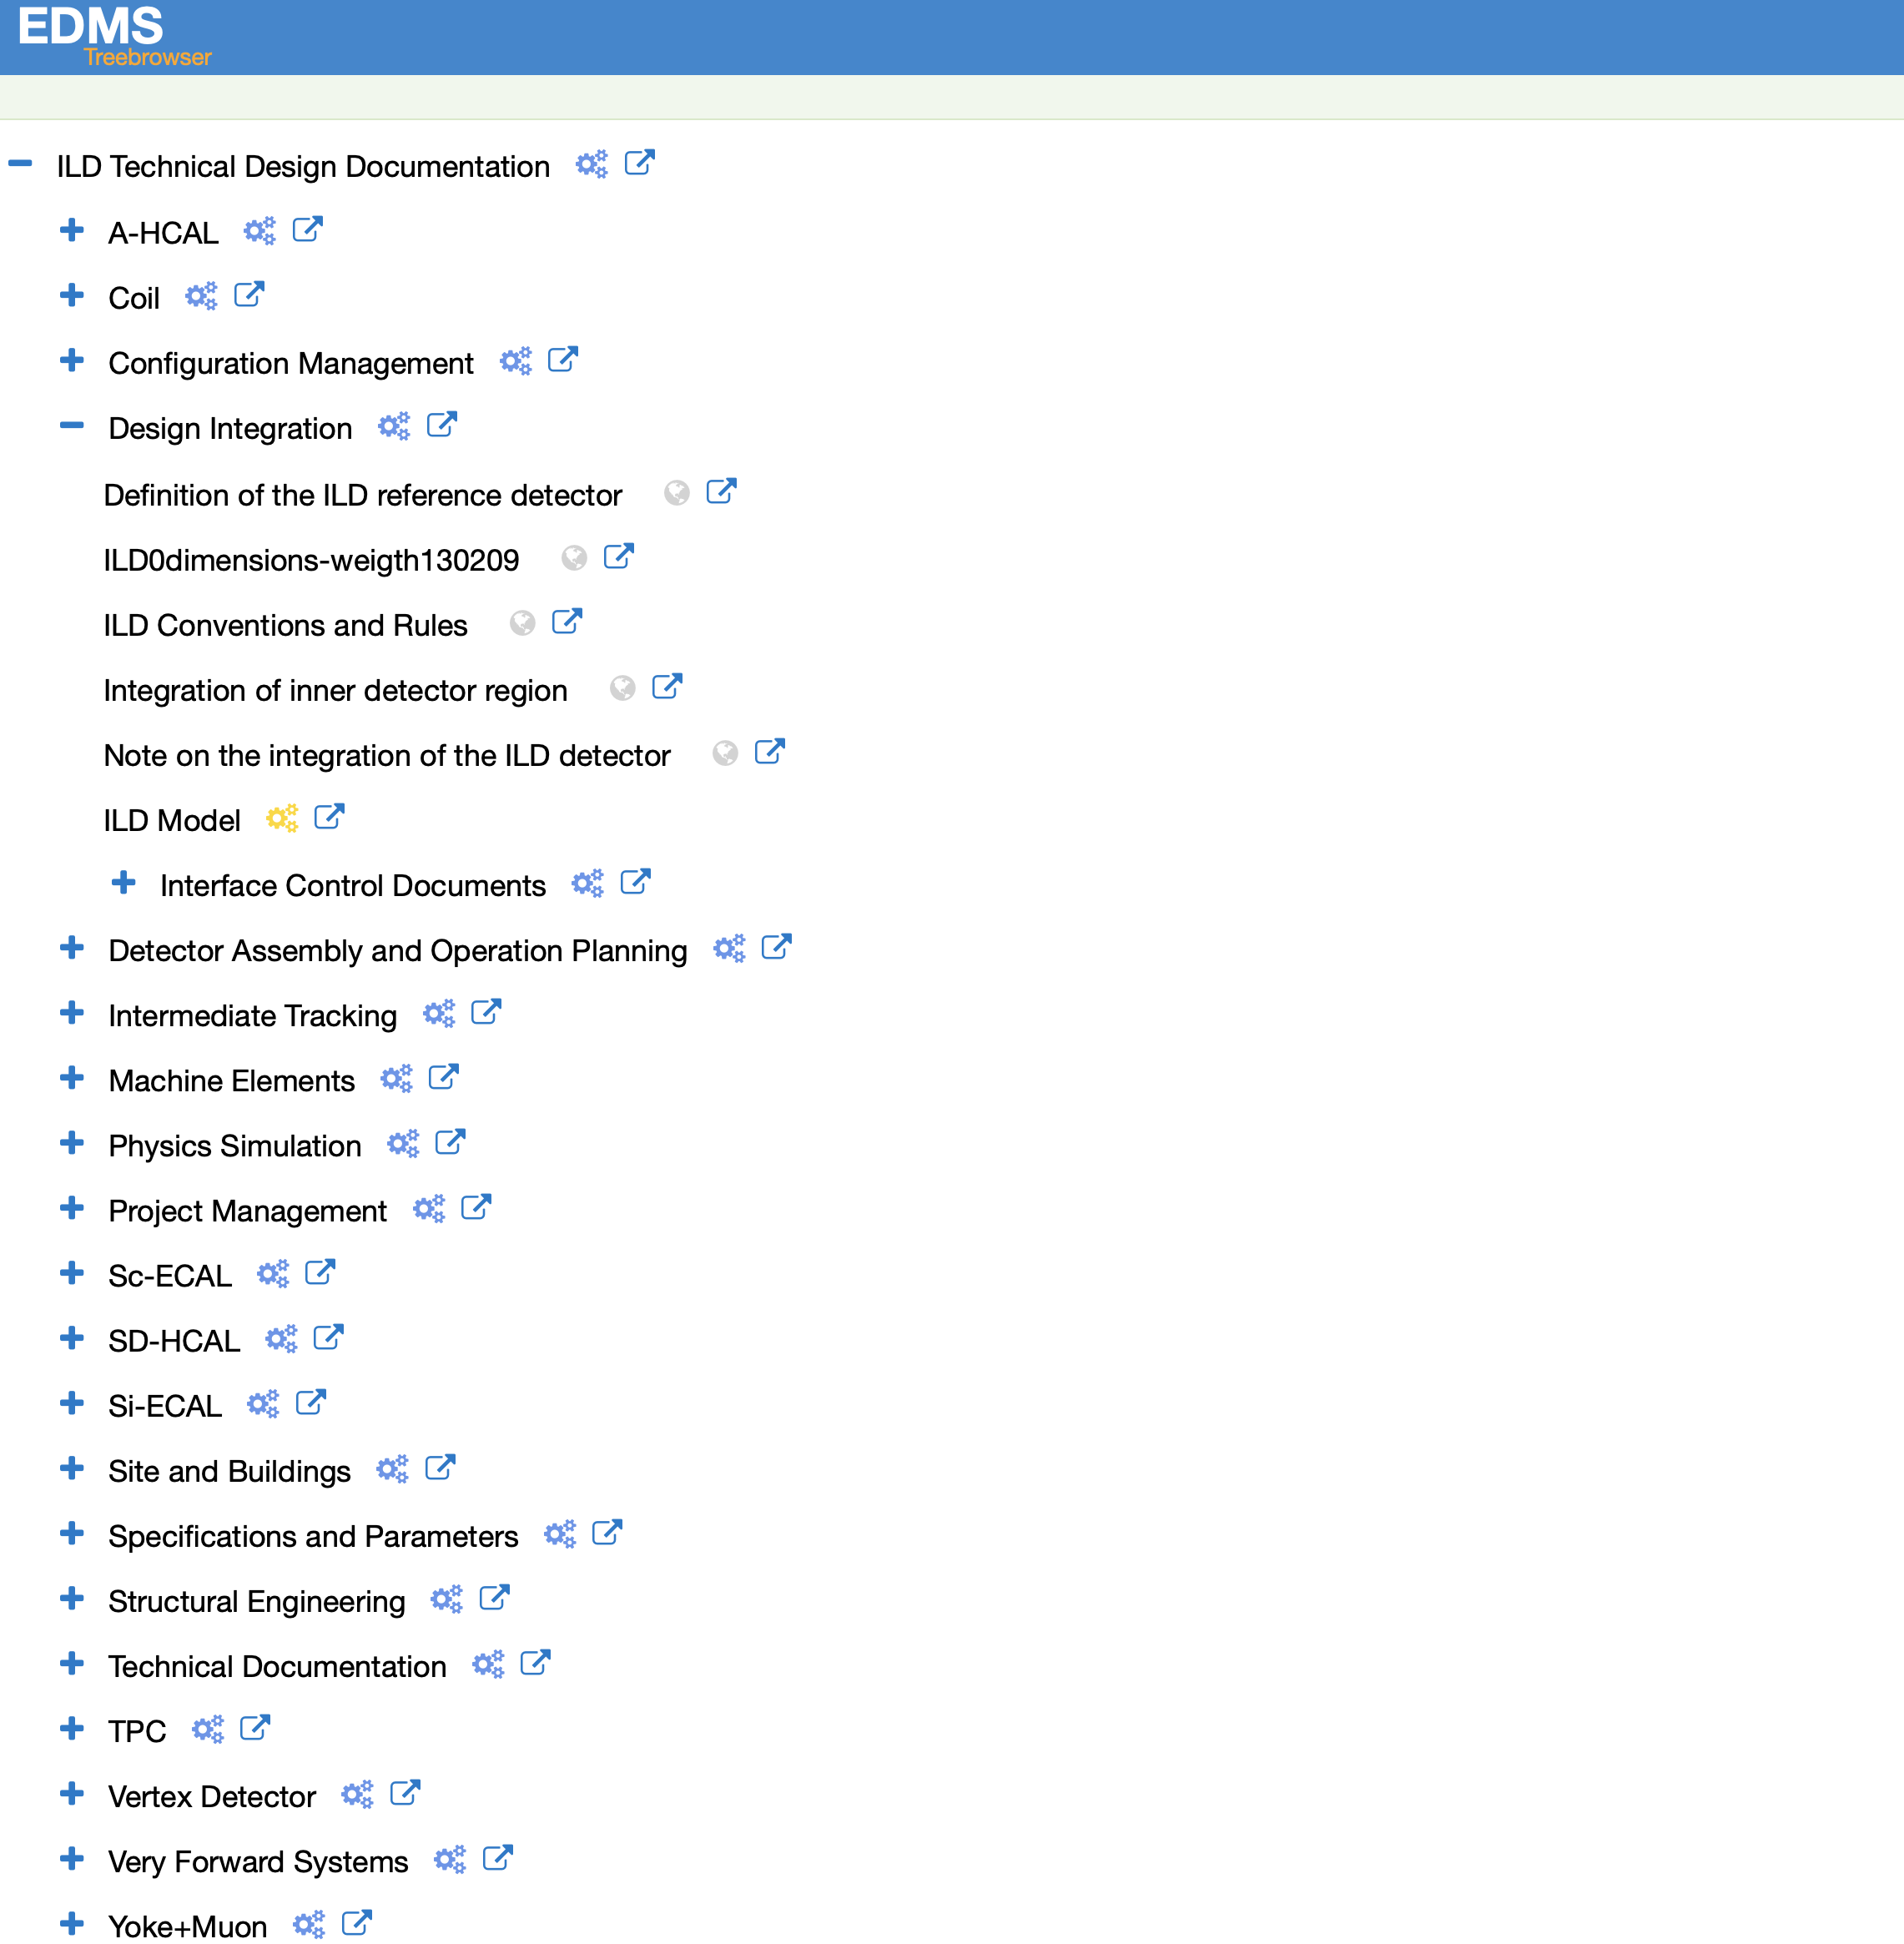
\includegraphics[width=0.8\hsize]{Integration/fig/EDMS_direct.png}

\caption{\label{ild:fig:integration:edmsdirect}Part of the treebrowser of the ILD technical documentation Work Breakdown Structure in the ILC Engineering Data Management System. The top level node "Design Integration" is shown expanded.}
\end{figure}

Figure~\ref{ild:fig:integration:edmsdirect_document} shows the document browser that opens for the documents stored in the EDMSdirect system. Shown here is the "Conventions and Rules" document that belongs to the previous mentioned WBS node "Design Integration". A preview of the document is shown in the document browser. The document browser allows for preview of the respective documents as well as downloads of pdf or source files, depending on the authorisation of the users. Documents can be made worldwide visible as well as protected for selected users.

\begin{figure}[h!]
\centering
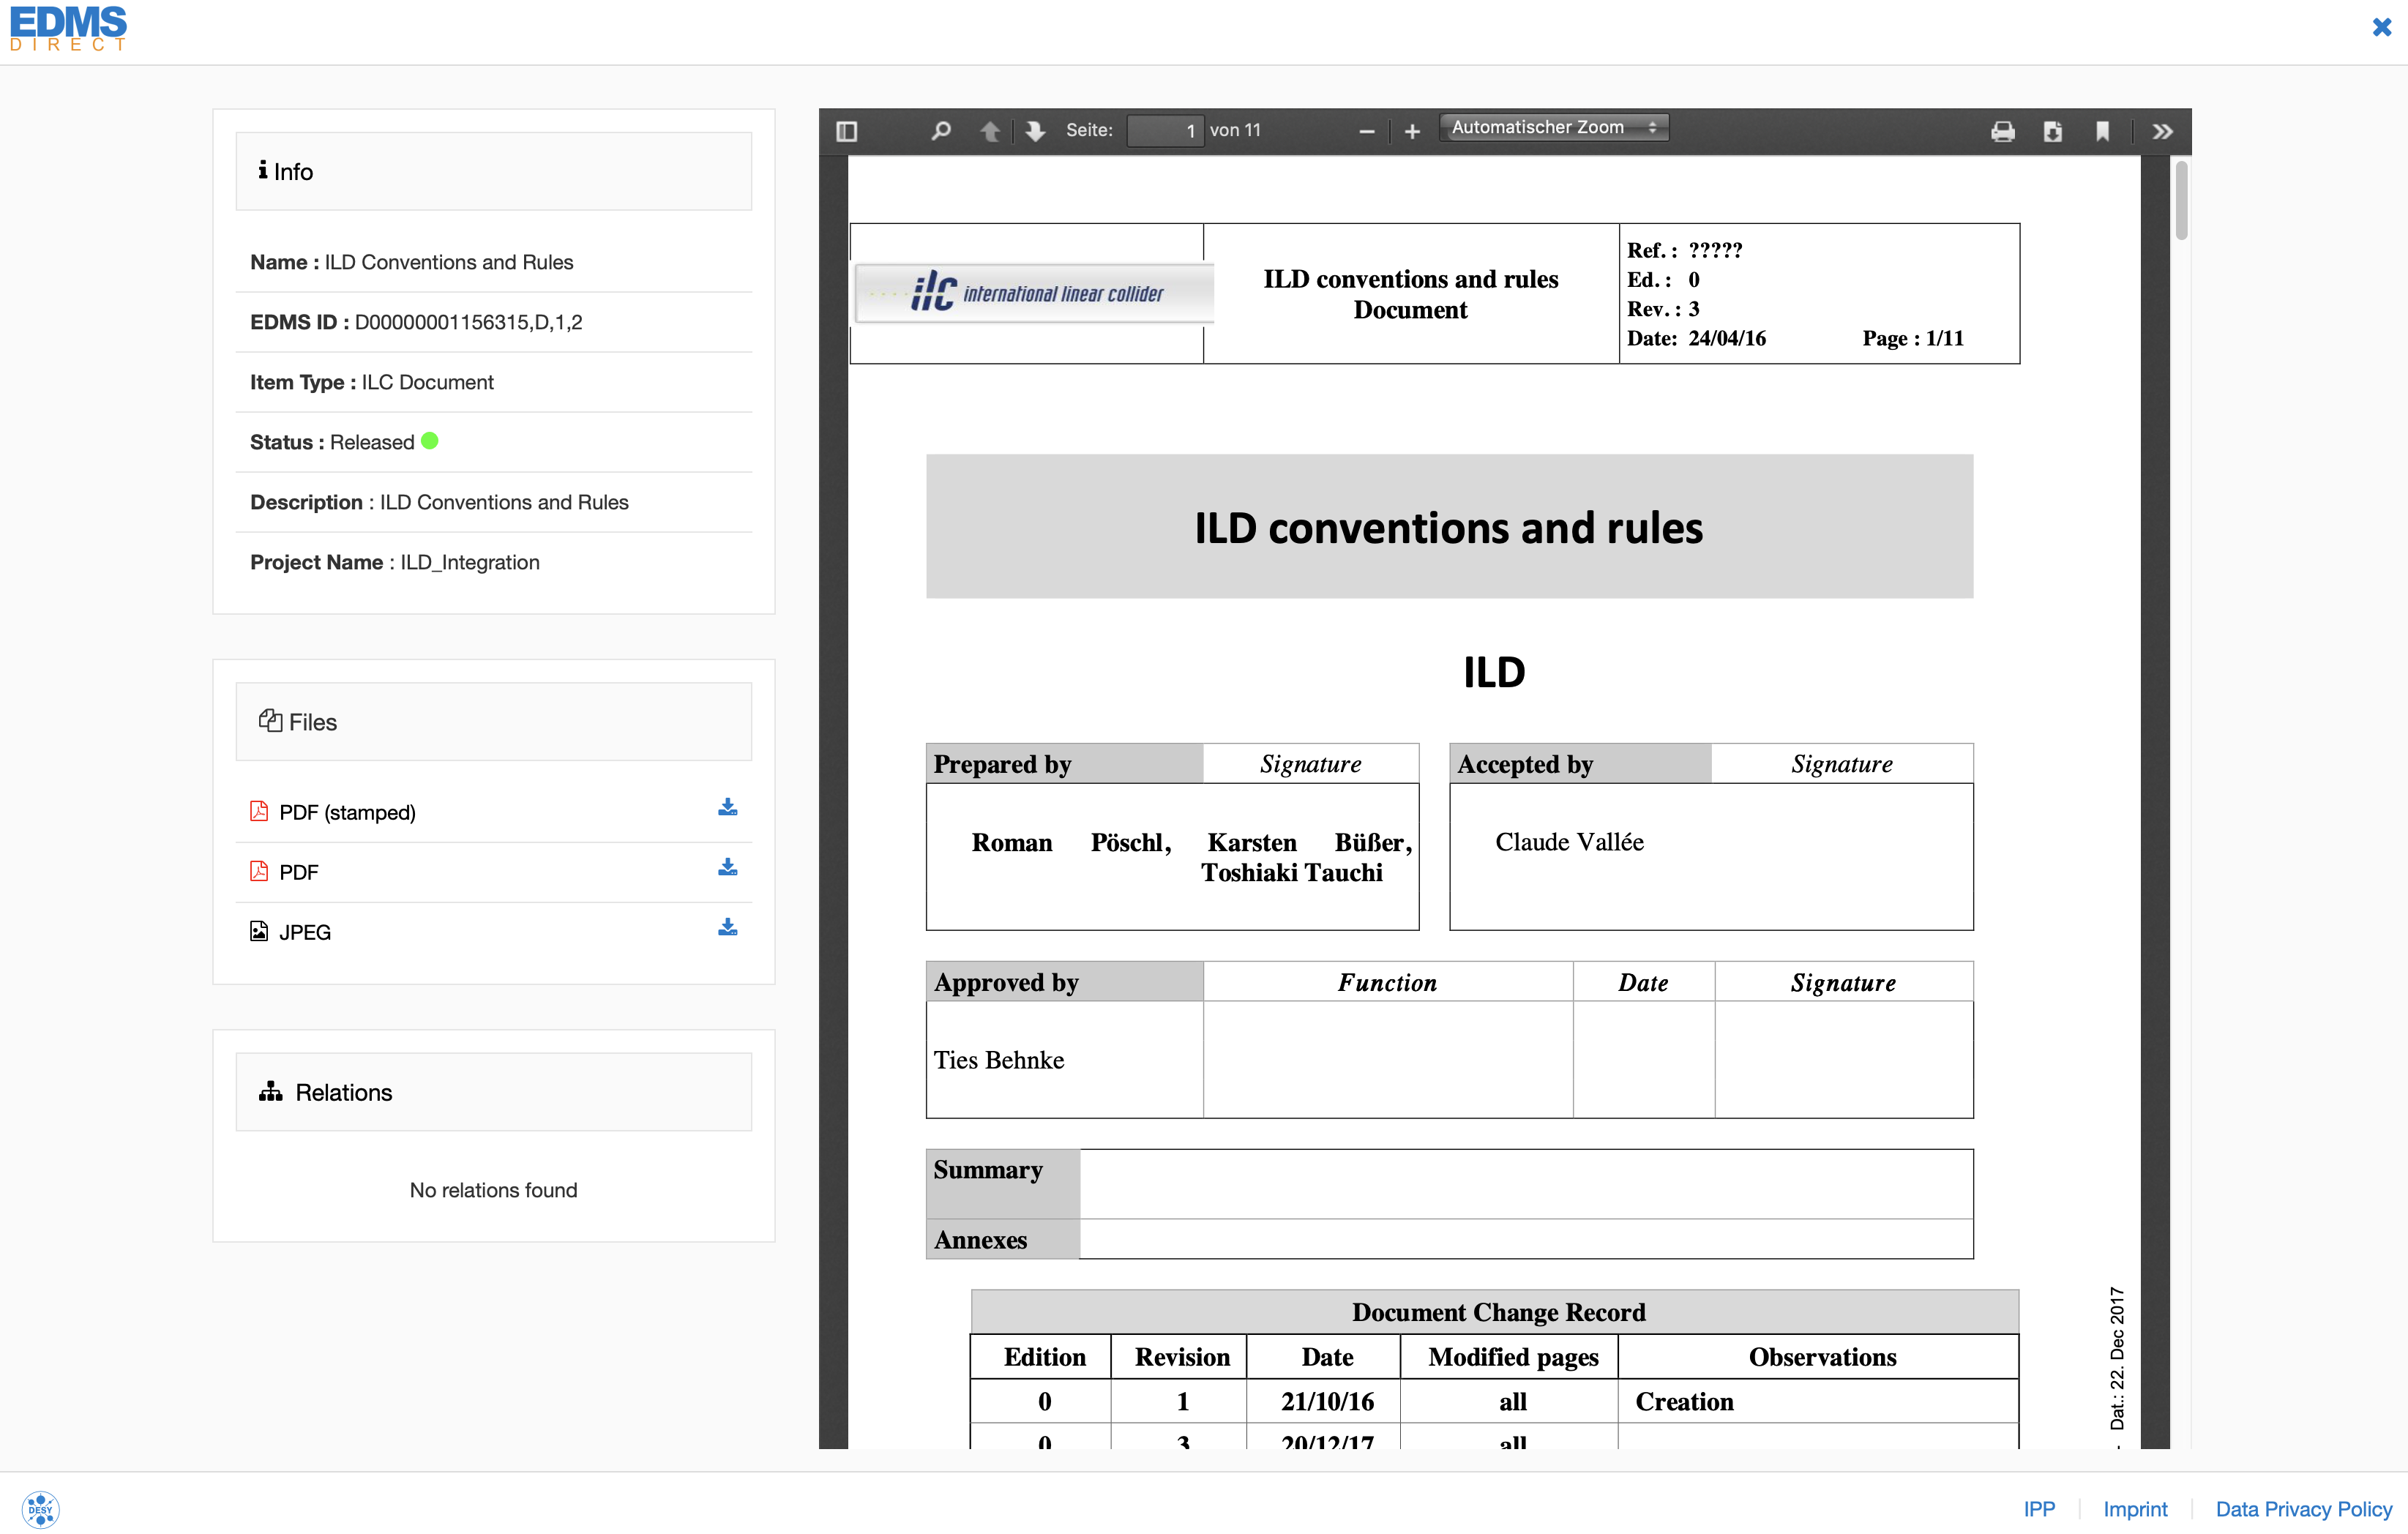
\includegraphics[width=0.8\hsize]{Integration/fig/EDMS_direct_document.png}

\caption{\label{ild:fig:integration:edmsdirect_document}Example document (here:"ILD Conventions and Rules") in the document browser of EDMSdirect.}
\end{figure}

\subsection{Interface Control Documents}
The technical integration of the ILD detector is based on a set of Interface Control Documents which describe the interfaces of each subdetector to its environment:
\begin{itemize}
    \item Mechanical Interface
    \begin{itemize}
        \item Local coordinate system
        \item Mechanical concept
        \item Critical dimensions
        \item Weights
        \item Positioning and alignment constraints
    \end{itemize}
    \item Electrical Interface
    \begin{itemize}
        \item Block and connection diagrams
        \item List of connectors
        \item Cabling and connection sheets
        \item Grounding circuits
        \item Power consumption
    \end{itemize}
    \item Gas and Liquid Interfaces
    \item Thermal Interfaces
    \item Test Interfaces
\end{itemize}
The Interface Control Documents are living documents that are updated as the design and understanding of the subdetector technologies advance. All documents are stored in EDMS~\cite{ild:bib:edms} and are accessible via the treebrowser of the ILD technical documentation~\cite{ild:bib:edmsdirect}.

A dedicated document describes the ILD Conventions and Rules (c.f.~figure~\ref{ild:fig:integration:edmsdirect_document}). It contains a definition of the global ILD coordinate system, unit conventions, naming and numbering conventions as well as mechanical, electrical and cooling constraints and rules. This document is also available on~\cite{ild:bib:edmsdirect}. 

The interface descriptions together with the conventions and rules contain the information that has been used in creating the integrated model of the ILD detector.